\documentclass[12pt,oneside]{book}

\usepackage[dvips,letterpaper,margin=0.75in,bottom=0.75in]{geometry}
\usepackage{cite}
\usepackage{slashed}
\usepackage{graphicx}
\usepackage{amsmath}
\usepackage{enumitem}

\usepackage[american,fulldiode]{circuitikz}
\tikzset{component/.style={draw,thick,circle,fill=white,minimum size =0.75cm,inner sep=0pt}}

\begin{document}
\ctikzset{bipoles/thickness=1}
\ctikzset{bipoles/length=.6cm}

\title{Physics 116C Scientific Python Exercises}

\maketitle

\chapter{Introduction to Plotting}

\section{Introduction}
This exercise will introduce calculations and plotting techniques using
numpy arrays within Scientific Python.

\section{Plotting discrete data and continuous functions}

\begin{figure}[htbp]
\begin{center}
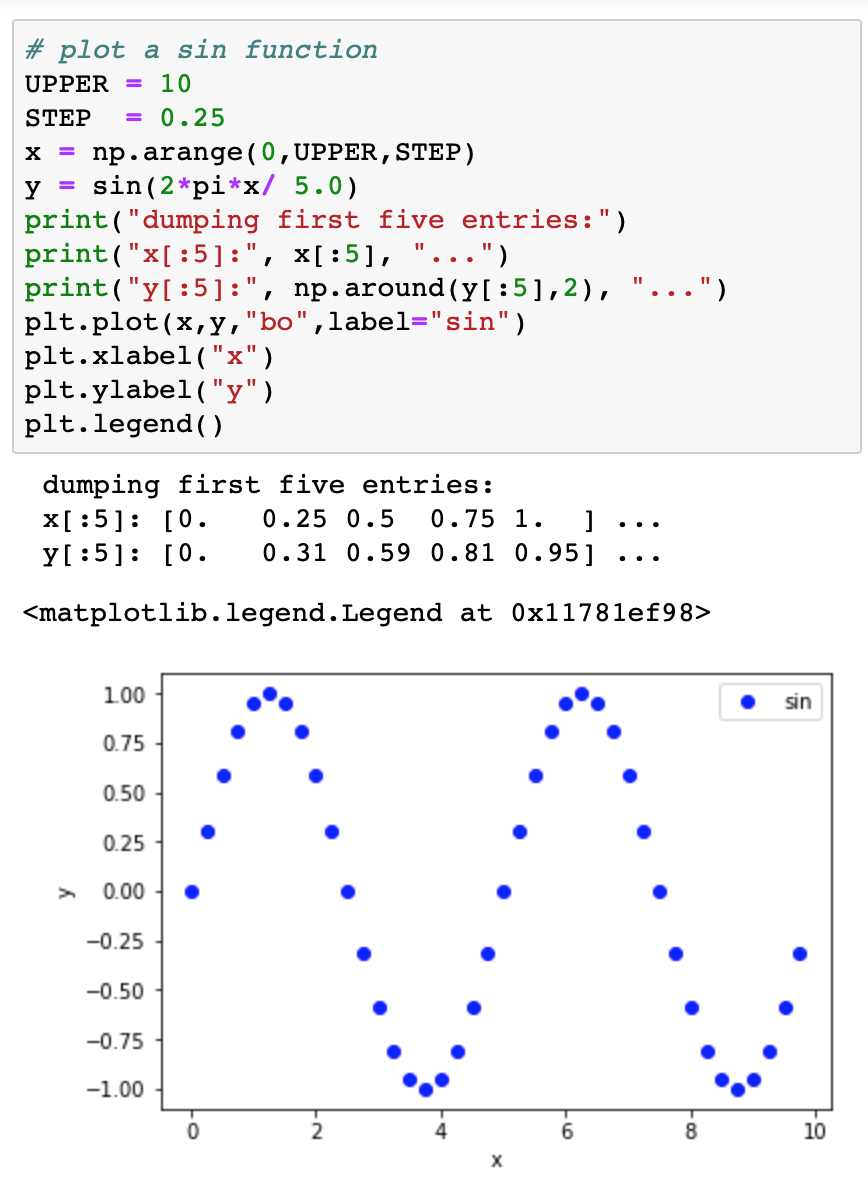
\includegraphics[width=0.65\textwidth]{figs//plotting/plotting.png} 
\caption{Circuit for verifying Ohm's law as a (a) circuit diagram, and (b) implemented using your lab equipment.}
\label{fig:plotsin}
\end{center}
\end{figure}

Consider the Jupyter notebook example in Fig.~\ref{fig:plotsin} which
plots a sine function sampled at discrete values.  Note the following
key features, which you will use repeatedly today and in future labs:
\begin{itemize}
\item Use of global variables {\tt UPPER} and {\tt STEP} at the top of
  the snippet, allowing for easy adjustment of parameters that affect
  the plot.
\item Use of {\tt np.arange} to define an array of x values.
\item Creation of the array y, defined by $y = \sin(2\pi x / 5)$ for each value of x.  One of the great joys of using numpy is the ability to avoid getting bogged down with explicit for loops.
\item Use of slicing techniques {\tt x[:5]} to show only the first five entries for debugging.  
\item Plotting the arrays of $x$ and $y$ values with {\tt plt.plot}  using the {\tt "bo"} option for blue circles.
\item Defining appropriate axis labels with {\tt plt.xlabel} and {\tt plt.xlabel}. 
\item Creation of a legend using the {\tt label} option to {\tt plt.plot} and the {plot.legend()} command.
\end{itemize}
Notice that even in this simple example, I've added some intermediate
feedback from my code in the form of the screen dumps of the first few
values of $x$ and $y$.  It's a common pitfall to try and rush ahead to
the final product when programming.  But it is much faster and
reliable to break your task into small steps, and establish feedback
at each small step.  To plot a continuous function with Scientific
Python, you will still use discrete data but:

\begin{itemize}
 \item Use much finer binning of the $x$-axis variable to draw a smooth curve. 
 \item Use the line option {\tt "-"} or dashed line {\tt "--"} instead of points with {\tt "o"}. 
\end{itemize} 

\noindent
{\bf Plot 1:}  Plot the quadratic function $y = x^2$ with the following requirements:
\begin{itemize}
 \item Plot in the range $x = [0,20)$.
 \item Plot discrete samples with a step size of $2$ using blue circles.
 \item On the same axis, plot the corresponding smooth function using a red solid line.
 \item Add appropriate axis labels. 
 \item Add a legend for the ``discrete'' and the ``smooth''  function.
\end{itemize}

\section{Multivariate analysis using boolean masks}
\begin{figure}[htbp]
\begin{center}
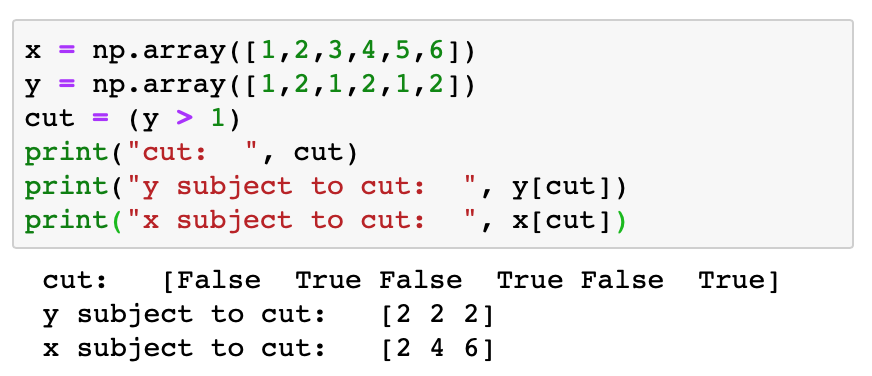
\includegraphics[width=0.65\textwidth]{figs//plotting/booleanmasks.png} 
\caption{Using boolean masks to cut on variable $y$.}
\label{fig:booleanmasks}
\end{center}
\end{figure}

A powerful technique in Scientific Python for performing analysis involving multiple variables uses boolean masks as shown in Fig.~\ref{fig:booleanmasks}.  In the example:
\begin{itemize}
\item Two numpy arrays $x$ and $y$ {\tt of the same length} are defined to contain the collected data.
\item The cut defined by $y > 1$ is a boolean array of the same length as $x$ and $y$ which is true at indices where the condition is met and false where it is not.
\item The subset of the entire $y$ array defined by {\tt y[cut]} consists only of those entries of $y$ for which the condition $y>1$ is met.
\item The subset of the entire $x$ array defined by {\tt x[cut]} consists only of those entries of $x$ for which the condition $y>1$ is met for the corresponding y value.
\end{itemize}
The last item shows the real power of this technique, one can look at one variable subject to constraints on another variable.

\begin{table}
\caption{Sample data for a voltage measurement subject to high frequency noise.}
\label{tbl:hfnoiseeg}
\begin{center}
\begin{tabular}{lll}
$t~(\rm s)$ & $v~(\rm V)$ & $n$ \\
0.4  & 0.25  &  2.8 \\
1.1  & 2.37  &  7.3 \\
1.4  & 1.69  &  9.7 \\
1.9  & 0.93  &  1.3 \\
2.5  & -1.0  &  6.2 \\
3.0  & 0.95  &  4.8 \\
3.4  & 1.22  &  6.9 \\
4.1  & 0.54  &  4.0 \\
4.4  & 0.37  &  1.9 \\
4.8  & 0.13  &  4.0 \\
5.5  & -2.04  &  9.5 \\
6.2  & -2.06  &  8.7 \\
6.5  & -0.81  &  2.3 \\
7.0  & -0.95  &  5.3 \\
7.5  & 0.98  &  9.7 \\
7.9  & 0.27  &  8.3 \\
8.5  & -0.81  &  0.1 \\
9.0  & -0.59  &  5.1 \\
9.4  & -0.37  &  4.4 \\
9.9  & 0.56  &  9.9 \\
\end{tabular}
\end{center}
\end{table}

Next consider the sample data in Table~\ref{tbl:hfnoiseeg} which comes from experimental measurements of a voltage level $v$ at discrete times $t$.  The measurement is subject to a high-frequency noise monitoring by the variable $n$.  The noise is only present for $n > 6.0$.  A straightforward way to load this data into scientific python is by defining numpy arrays for each variable as follows:
\begin{verbatim}
t = np.array([0.4, 1.1, 1.4, 1.9, 2.5, 3.0, 3.4, 4.1, 4.4, 4.8, 
                     5.5, 6.2, 6.5, 7.0, 7.5, 7.9, 8.5, 9.0, 9.4, 9.9])
v = np.array([ 0.25, 2.37, 1.69, 0.93, -1.0, 0.95, 1.22,   
                      0.54, 0.37, 0.13, -2.04, -2.06, -0.81, -0.95,  
                      0.98, 0.27, -0.81, -0.59, -0.37, 0.56])
n = np.array([2.8, 7.3, 9.7, 1.3, 6.2, 4.8, 6.9, 4.0, 1.9, 4.0,  
                      9.5, 8.7, 2.3, 5.3, 9.7, 8.3, 0.1, 5.1, 4.4, 9.9])
\end{verbatim}

\noindent
{\bf Plot 2} Prepare a plot of the sample data subject to the following:
\begin{itemize}
 \item Plot the voltage as a function of time as discrete data using red points.
 \item Define the boolean array {\tt keep} based on the noise reducing condition $n<=6.0$.
 \item Plot the voltage as a function of time, subject to the noise reducing condition using blue points.
 \item Plot the function $\sin(2 \pi x / 10)$ as a smooth function.
 \item Add appropriate axis labels.
 \item Add a legend for ``raw'' data with no cut, ``clean'' data with noise removed, and your continuous ``sin'' function.   
\end{itemize}
Your plot will reveal a clear sine function in the discrete data (after noise removal) consistent with the continuous function.  





\chapter{Histograms}

\section{Introduction}

In this exercise, you will learn how to produce and display
histograms, and compare histogram data with a distribution function.

\section{Histogram of Simulated Data}

First we will generate fake data, called Monte Carlo data, in order to
have something to plot.  We'll use the {\tt random.norm} function to
produce 200 events randomly drawn from a Gaussian distribution with
mean of 5, and sigma of 1.5:
\begin{center}
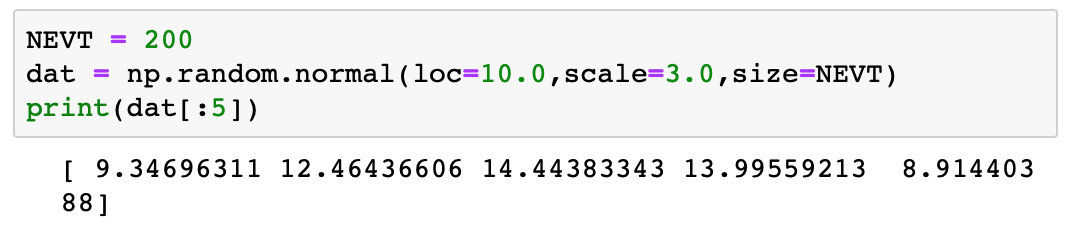
\includegraphics[width=0.85\textwidth]{figs/histograms/mc.png}\\ 
\end{center}
Notice the scipy names for the Gaussian parameters are {\tt loc} for
the mean, and {\tt scale} for $\sigma$.  The first five events of the
200 produced are printed to the screen as a quick check of our work.

\begin{figure}[htbp]
\begin{center}
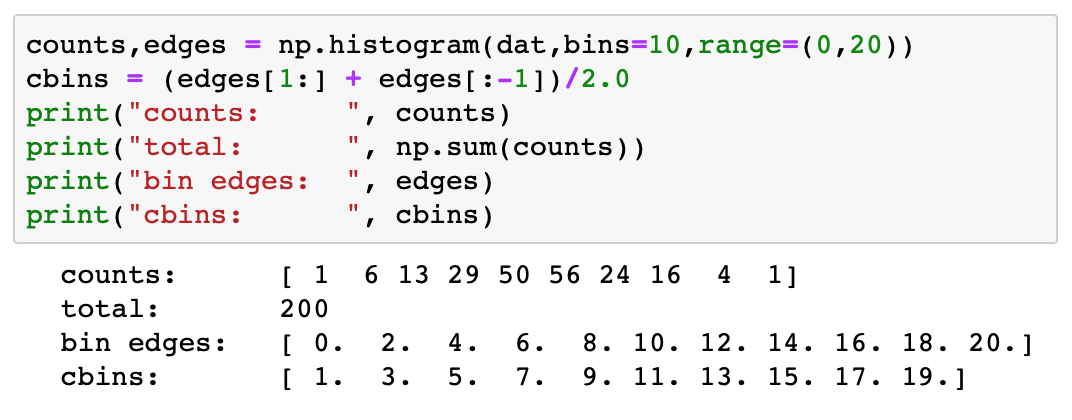
\includegraphics[width=0.85\textwidth]{figs/histograms/hist.png} 
\end{center}
\caption{\label{fig:hist} Example creating a histogram.}
\end{figure}

Next we'll produce a histogram for this simulated data, as shown in
Fig.~\ref{fig:hist} using the scipy {\tt histogram} function:
\begin{verbatim}
counts,edges = np.histogram(dat,bins=10,range=(0,20))
\end{verbatim}
where we have specified 10 bins, uniformly covering the range from 0
to 20.  The function returns to arrays, which we save as {\tt counts}
and {\tt edges}.  The {\tt counts} array contains the bin contents,
the count of the number of values in each bin:
\begin{verbatim}
counts:      [ 1  6 13 29 50 56 24 16  4  1]
\end{verbatim}
The edges array contains the edges of the bins:
\begin{verbatim}
bin edges:   [ 0.  2.  4.  6.  8. 10. 12. 14. 16. 18. 20.]
\end{verbatim}
You'll notice that 10 consecutive bins have 11 edges.  When plotting continuous data, plot the contents at the center of each bin:
\begin{verbatim}
cbins = (edges[:-1] + edges[1:])/2.0
\end{verbatim}
Here the two slices {\tt edges[:-1]} and {\tt edges[1:]} are all but the last and all but the first edges.  The average of the two is the center of each bin:
\begin{verbatim}
cbins:    [ 1.  3.  5.  7.  9. 11. 13. 15. 17. 19.]
\end{verbatim}

We can take a quick look at the histogram data with the {\tt plot} function:
\begin{center}
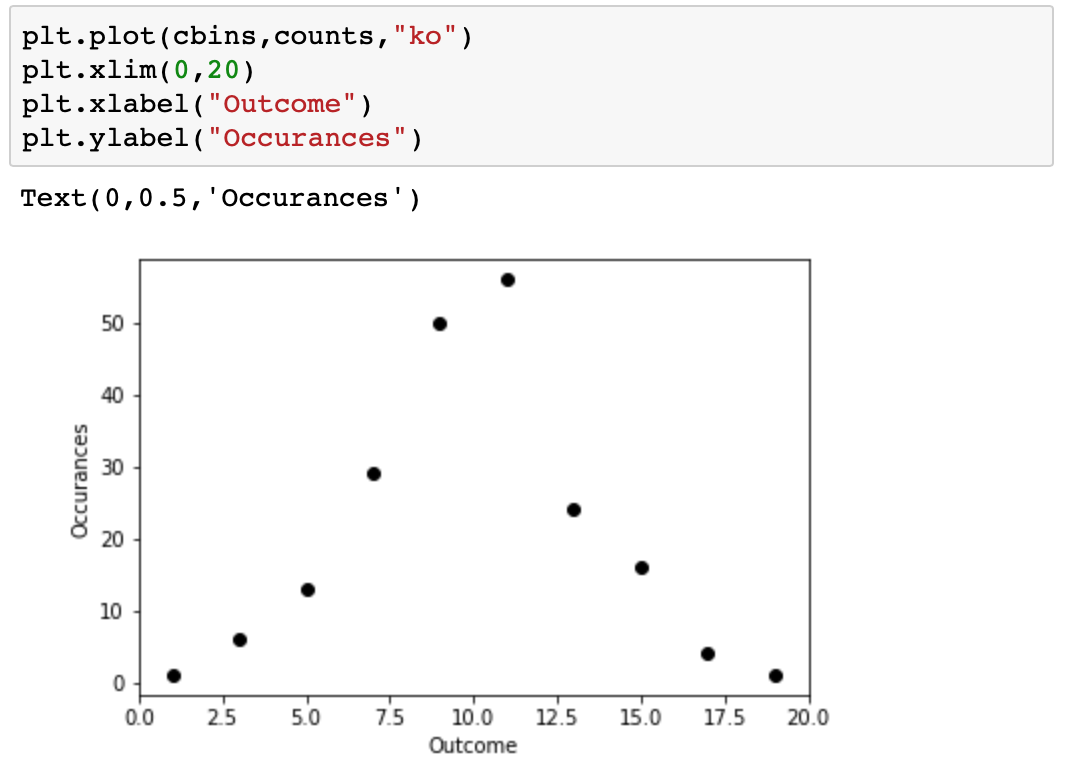
\includegraphics[width=0.85\textwidth]{figs/histograms/plot.png}\\ 
\end{center}

The content of each bin is a single number, a count, and is therefore
subject to the Poisson distribution.  We can estimate the mean of the
Poisson distribution by the measured value, so that $\lambda = N$.
For the Poisson distribution, the variance $\sigma^2 = \lambda$, and
so $\sigma = \sqrt{N}$.  It is customary to draw a line of size
$\sqrt{N}$ when plotting a histogram value $N$. This is an example of
an error bar, which indicates how well our measurement has determined
a particular value.
\begin{center}
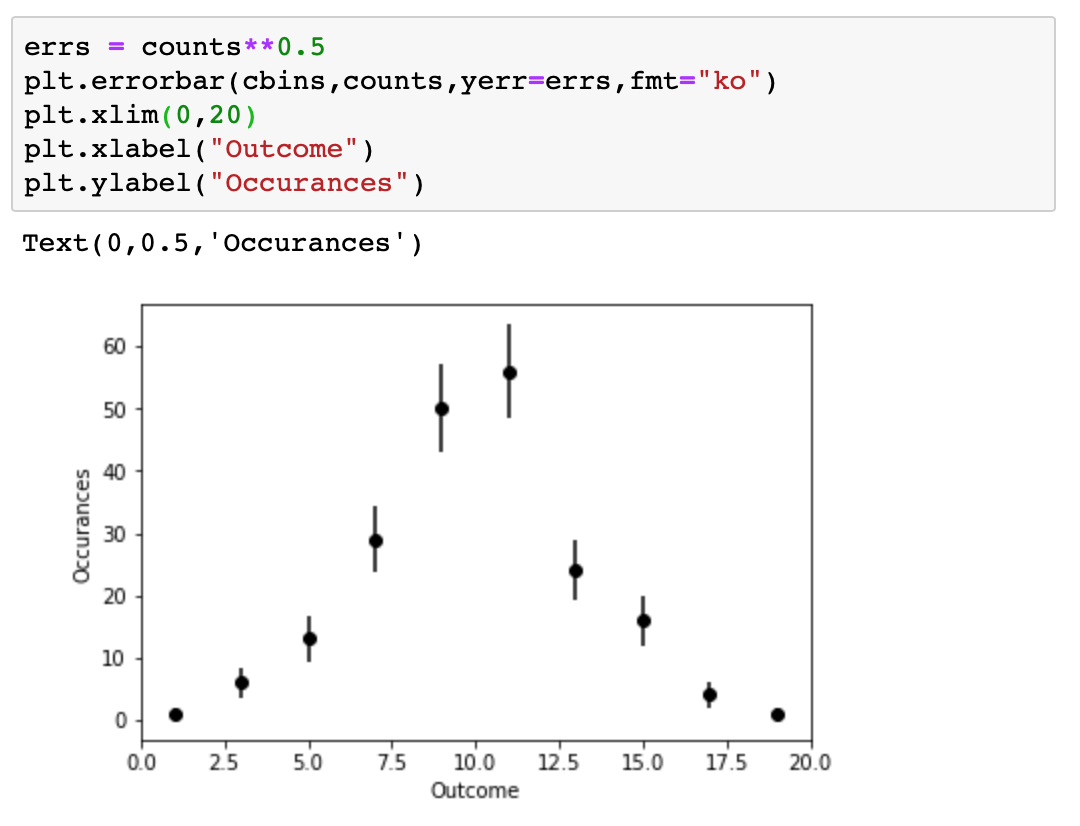
\includegraphics[width=0.85\textwidth]{figs/histograms/err.png}\\ 
\end{center}

\section{Comparison to Distribution Function}

\begin{figure}[htbp]
\begin{center}
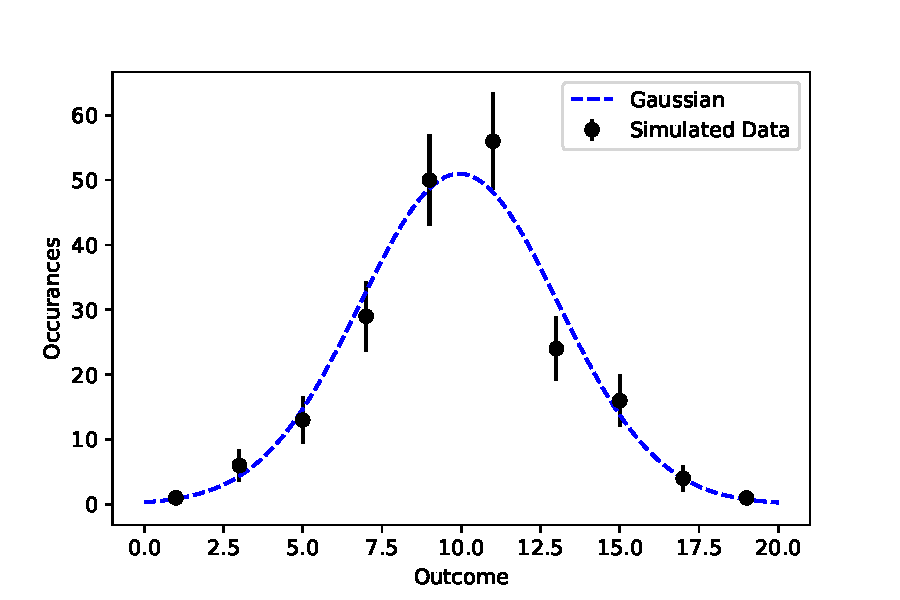
\includegraphics[width=0.7\textwidth]{figs/histograms/gaussian_eg.pdf} 
\end{center}
\caption{\label{fig:gauss} Comparison of simulated data to Guassian PDF.}
\end{figure}

Our theoretical models often predict a PDF for some observable
variable $x$.  As experimentalists, we are often therefore concerned
with the question as to whether our collected data for an observable
$x$ is consistent with the theoretical PDF.  A visual approach to
answering this question is to plot the data in a histogram, and to
draw the PDF as a curve normalized to the histogram.

To predict the number of events in a bin with edges $x_{\rm lower}$
and $x_{\rm upper}$, in principle we need to integrate the PDF and
normalize to the number of experiments:
\begin{displaymath}
N_{\rm pred} = N_{\rm meas} \int^{x_{\rm upper}}_{x_{\rm lower}} p(x) \, dx
\end{displaymath}
In practice, we generally choose the bin sizes small enough that the
PDF is approximately constant during the entire bin, and in this case,
the prediction can be taken as:
\begin{displaymath}
N_{\rm pred} = N_{\rm meas} \; \Delta x \; p(x)
\end{displaymath}
where $\Delta x$ is the width of each bin.  This scale factor $N_{\rm
  meas} \; \Delta x$ allows us to compare a continuous function to
data accumulated within bins.

{\bf Plot 1:} Reproduce the plot in Fig.~\ref{fig:gauss} by comparing
the simulated data to the Gaussian distribution function available
from the {stats.norm.pdf} function.  To use the {\tt stats} library, you will need to import it:
\begin{verbatim}
from scipy import stats
\end{verbatim}
You'll need to appropriately scale the PDF.


{\bf Plot 2:}  Repeat the plot with 10,000 events and 50 bins in the range from $(0,20)$.
















\chapter{Curve Fitting}
%ADD CHI2 calculation 
\section{Introduction}

In this lab, you will learn about curve fitting with Scientific Python
function {\tt curve{\_}fit}.  For this lab there are only jupyter notebook entries. 

Given a function to fit $f(x;p)$, with p
representing any number of parameters, and a set of measurements $y_i$ and points $x_i$,
the {\tt curve{\_}fit} function determines the best fit parameters by
minimizing:
\begin{equation}
\chi^2 = \sum_i \frac{(f(x_i;p) - y_i) ^2}{\sigma_i^2}.
\label{eqn:chi2}
\end{equation}
If the uncertainties $\sigma_i$ are not specified, the function
assumes $\sigma_i = 1$, and still finds the correct minimum
if the actual uncertainties are identical to one another.

\section{Fitting a Straight Line}

\begin{figure}[htbp]
\begin{center}
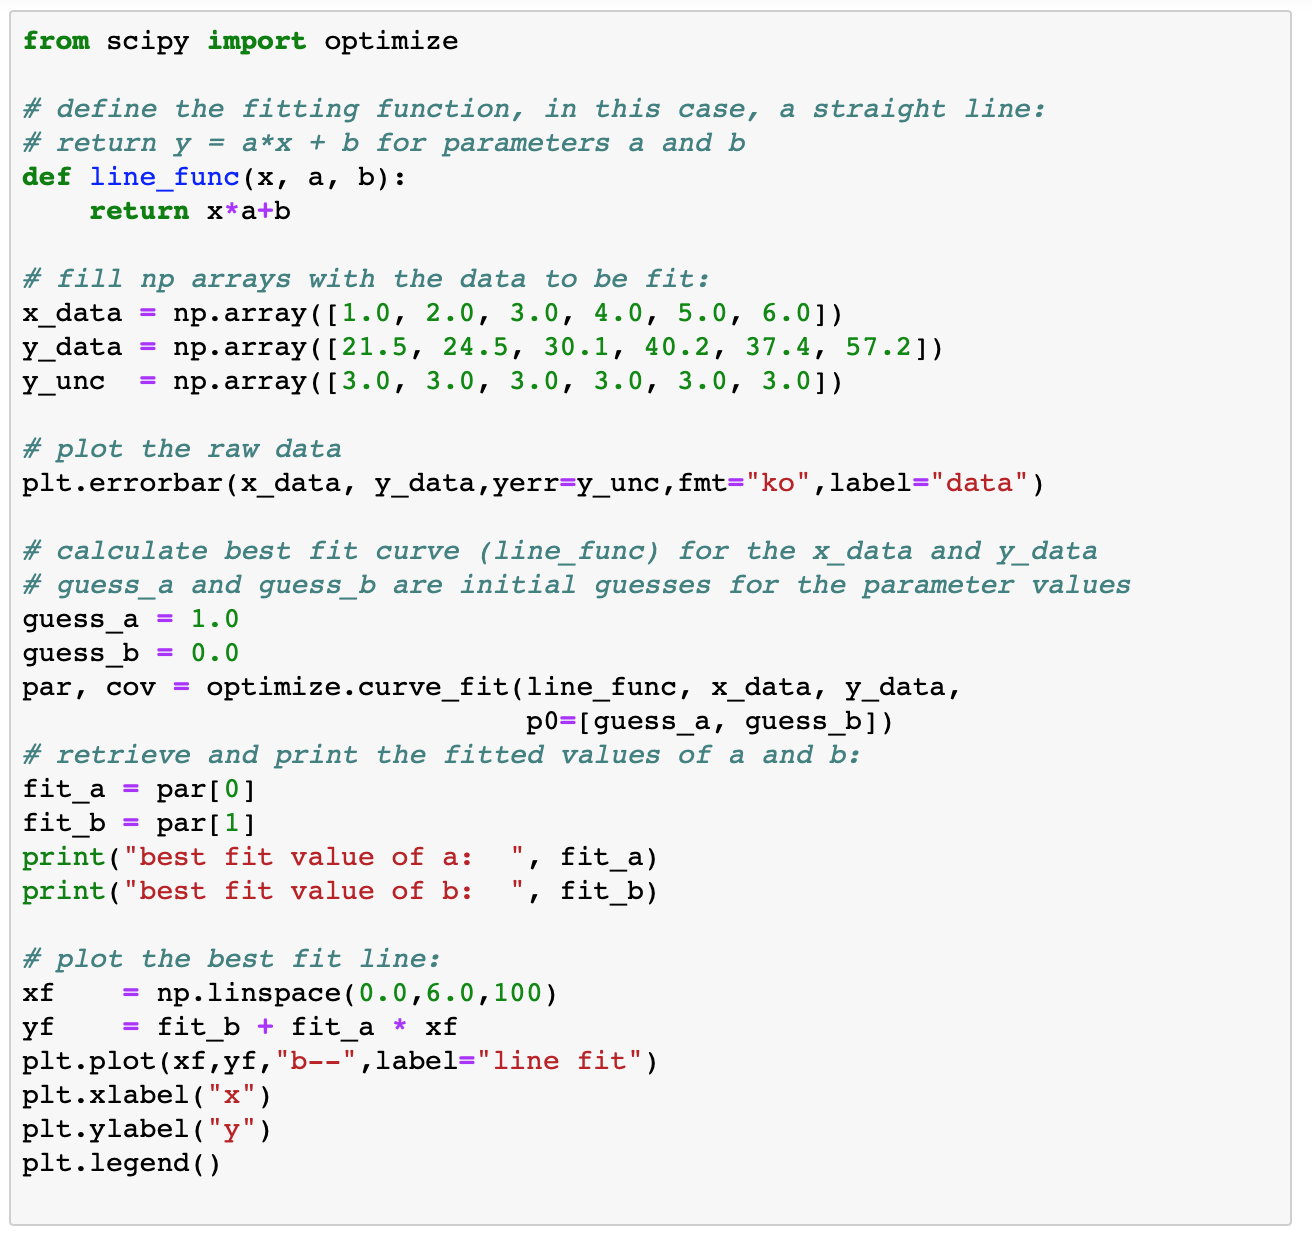
\includegraphics[width=0.65\textwidth]{figs/labs/fitting/fit_code.png} \\
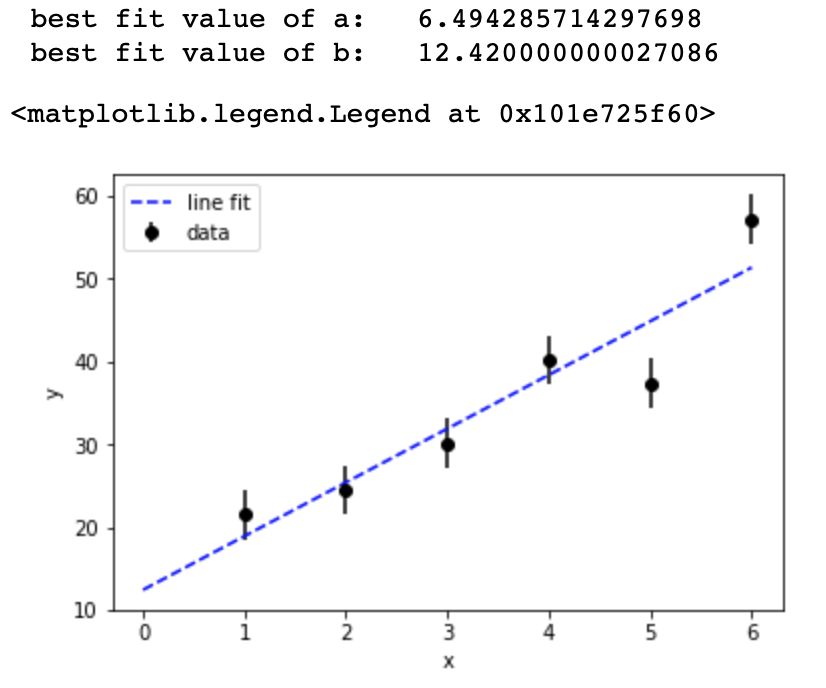
\includegraphics[width=0.65\textwidth]{figs/labs/fitting/fit_out.png} \\
\caption{Example fitting data to straight line.}
\label{fig:fiteg}
\end{center}
\end{figure}

An example using Scientific Pythons {\tt curve{\_}fit} function to fit
a straight line to data is shown in Fig.~\ref{fig:fiteg}.  A block of 
code defining the function we wish to fit, in this case, a straight
line, is defined as a function:
\begin{verbatim}
     def line_func(x, a, b):
         return a*x + b
\end{verbatim}
In this case, the function requires three parameters (in the computer
science sense) the x data in a numpy array as function parameter x,
the slope as function parameter a, and the intercept as function
parameter b.  When called, the function returns the x data multiplied
by the value a, with the value b added.  We don't directly call this
function, but in principle, it could be called like:
\begin{verbatim}
    y_data = line_func(x_data, 2.0, 0.0)
\end{verbatim}
to create a numpy array {\tt y{\_}data} constructed from {\tt
  x{\_}data} with slope 2 and intercept 0.

The next section filling numpy arrays containing the data, and
plotting it with error bars should be familiar by now.  The fit itself
is performed by the line:
\begin{verbatim}
par, cov = optimize.curve_fit(line_func, x_data, y_data, p0=[guess_a, guess_b])
\end{verbatim}
This performs a fit of the function {\tt line{\_}func} defined above
to the $x$ and $y$ data contained in the arrays {\tt x{\_}data} and
{\tt y{\_}data}.  Numerical fits generally find the local minimum,
which is not necessarily the global minimum of interest.  It is
important therefore, especially for complicated fits, to provide an
initial guess near the expected fit values.  These are provided to the
optional, named, function parameter {\tt p0}, which is set to the
python list {\tt [guess{\_}a, guess{\_}b]} which contains our initial guesses for
the fit parameters $a$ and $b$.  The function performs a least-squares
fit to find the best values of $a$ and $b$ which are returned as the
numpy array {\tt par}.  The function also returns the covariance
matrix as the numpy array {\tt cov}.

The remaining code simply uses the best fit values to plot the fitted
function as a dashed line.  Numerical fits are fickle.  Even if you
are only interested in the fitted value, you should always plot the
best-fit function and compare the results to your data as in important
check for your work.

\begin{table}
\caption{Sample data for straight line fit.}
\label{tbl:linesamp}
\begin{center}
\begin{tabular}{ll}
$x$ & $y \pm \sigma_y$ \\
1.0  & $15.9 \pm 3.0$ \\
2.0  & $23.6 \pm 3.0$ \\
3.0  & $33.9 \pm 3.0$ \\
4.0  & $39.7 \pm 3.0$ \\
5.0  & $45.0 \pm 10.0$ \\
6.0  & $32.4 \pm 20.0$ \\
\end{tabular}
\end{center}
\end{table}

%\begin{figure}[htbp]
%\begin{center}
%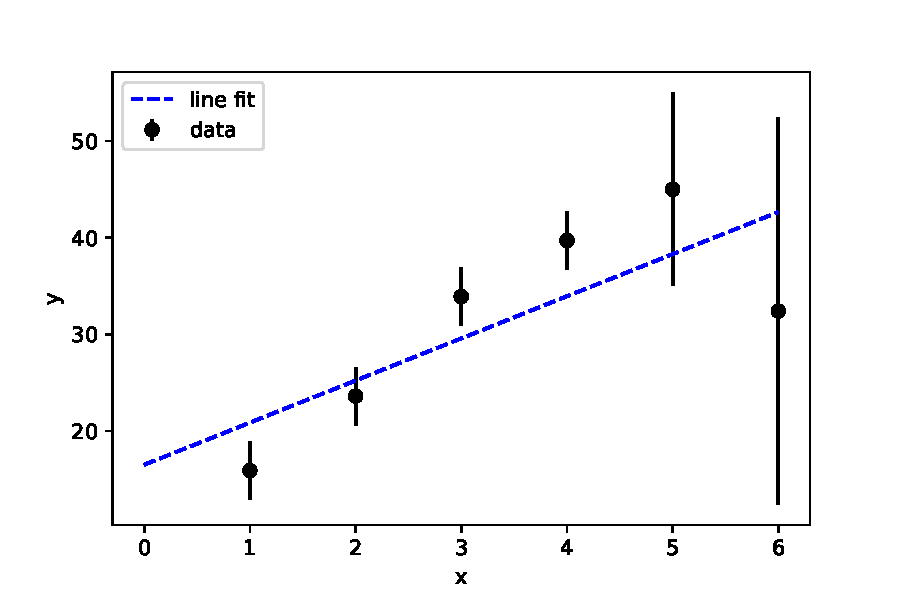
\includegraphics[width=0.65\textwidth]{figs/labs/fitting/bias.pdf} 
%\caption{This linear fit is biased by the failure to properly account for uncertainties.}
%\label{fig:fitbias}
%\end{center}
%\end{figure}

\begin{plot} Apply a code like that of Fig.~\ref{fig:fiteg}
to the data in Table~\ref{tbl:linesamp}. Plot the data including error bars and the best-fit function.
% reproduce the plot in Fig.~\ref{fig:fitbias}.  
\end{plot}

Notice that the last two data points have larger uncertainties than
the other data points.  However, the call to the {curve{\_}fit}
function does not provide the parameter uncertainties, and so the
function assumes that they all have the value $1$.  In this case,
since the uncertainties are not in fact all the same, the function
does not find the correct minimum.  The answer is clearly biased
toward the poorly measured points, because the function gives these
points the same weight as all of the other points.

\begin{print} The {\tt curve{\_}fit} function does not provide directly the $\chi^2$ value of the fit. However you can calculate it manually via equation~\ref{eqn:chi2}. The sum can be obtained via numpy function sum. Modify your code to include calculation of the $\chi^2$ value of the fit. Include also the calculation of the $\chi^2$ divided by the number of degrees of freedom (number of data points minus number of parameters), which is called reduced $\chi^2$. Print both of those values. Is the fit reasonable based on the reduced $\chi^2$ value? Print your comment as well. 
\end{print}

\begin{plot} Look-up the {\tt curve{\_}fit} function and the optional parameter
{\tt sigma}. Provide the correct uncertainties to
the fit and make a new plot with the data and the fit.  You should observe that the fit results is no longer biased,
and more closely tracks the well constrained left side of the plot. \end{plot}

\begin{print} Print $\chi^2$ and reduced $\chi^2$ value. Is the fit reasonable based on the reduced $\chi^2$ value? Print your comment as well. \end{print}

\section{Parameter Uncertainties I}
\label{sec:sigmatrue}
As discussed in the lecture the uncertainty $\sigma_{p_i}$ on the $i$th parameter $p_i$
can be determined from the second derivative of the $\chi^2$ function:
\begin{displaymath}
\frac{d^2\chi^2}{d p_i^2} = \frac{2}{\sigma_{p_i}^2}.
\end{displaymath}
In general, for $M$ parameters, the $M \times M$ covariance matrix is calculated as:
\begin{displaymath}
C(i,j) = 2 \cdot \left(\dfrac{d^2\chi^2}{d p_i d p_j} \right)^{-1}
\end{displaymath}
from which we can see that the diagonals are simply the parameter uncertainties squared:
\begin{displaymath}
C(i,i) = 2 \cdot \left(\dfrac{d^2\chi^2}{d p_i^2} \right)^{-1} = \sigma^2_{p_i}.
\end{displaymath}
The off-diagonal elements contain information about how parameters are
correlated, and for a well designed fit function they should be close to
zero.

The {\tt curve{\_}fit} function returns both the best fit parameter values and the covariance matrix:
\begin{verbatim}
par, cov = optimize.curve_fit(...)
\end{verbatim}
For a fit with $M$ parameters, we can obtain an array containing the
$M$ parameter uncertainties from the square root of the diagonals of the $M \times M$
covariance matrix:
\begin{verbatim}
unc = np.sqrt(np.diag(cov))
\end{verbatim}

We can obtain uncertainties of parameters by accessing elements of the array.

Lets study this in an example for $N=1$ parameter. Generate $x$-values as a numpy array of evenly spaced values from 0 to 99. Generate $y$-values as 100 random numbers drawn from a Gaussian distribution with mean $m = 50$ and a width $\sigma_y =10$.  Perform a fit using {\tt curve{\_}fit} function. Set the uncertainties on the $y$ values to 10 and also set parameter {\tt absolute{\_}sigma = True}.  

 The best fit constant value we expect is simply the mean of the $y$-values.  The
uncertainty on the mean value should be:
\begin{displaymath}
\sigma_m = \sigma_y / \sqrt{N} = 10 / \sqrt{100} = 1.0
\end{displaymath}

\begin{print} Calculate the expected values for the best fit value and its uncertainty. Print them together with the fitted best fit value and its uncertainty. Do those agree? \end{print}


\section{Fitting a Sine Curve}

In this section, you will fit the sample data to a sine function:
\begin{displaymath}
 y = A \, \sin( k x). 
\end{displaymath}
Use the following sample data:\\
\begin{center}
\begin{tabular}{|ll| ll|ll|}
\hline
$x$ & $y$ & $x$ & $y$ & $x$ & $y$\\
\hline
0  & 5.3    & 4  & -9.7   & 8  & 15.7  \\
1  & 15.0   & 5  & -17.4  & 9  & 18.5  \\
2  & 19.2   & 6  & -20.5  & 10 & 8.6   \\
3  & 6.8    & 7  &  2.1   & &  \\
\hline
\end{tabular}
\end{center}
Assume the uncertainty is the same for each $y$ value: $\sigma_i = 2$.
\begin{plot} Plot the data including error bars and the best-fit
sine wave. \end{plot}

\begin{print} Print the best fit parameter
values and their uncertainties. \end{print}

Remember to set {\tt absolute{\_}sigma=True}.\\

This is a \textbf{sign-off point} for this lab. 

\section{Parameter Uncertainties II}

%\begin{figure}[htbp]
%\begin{center}
%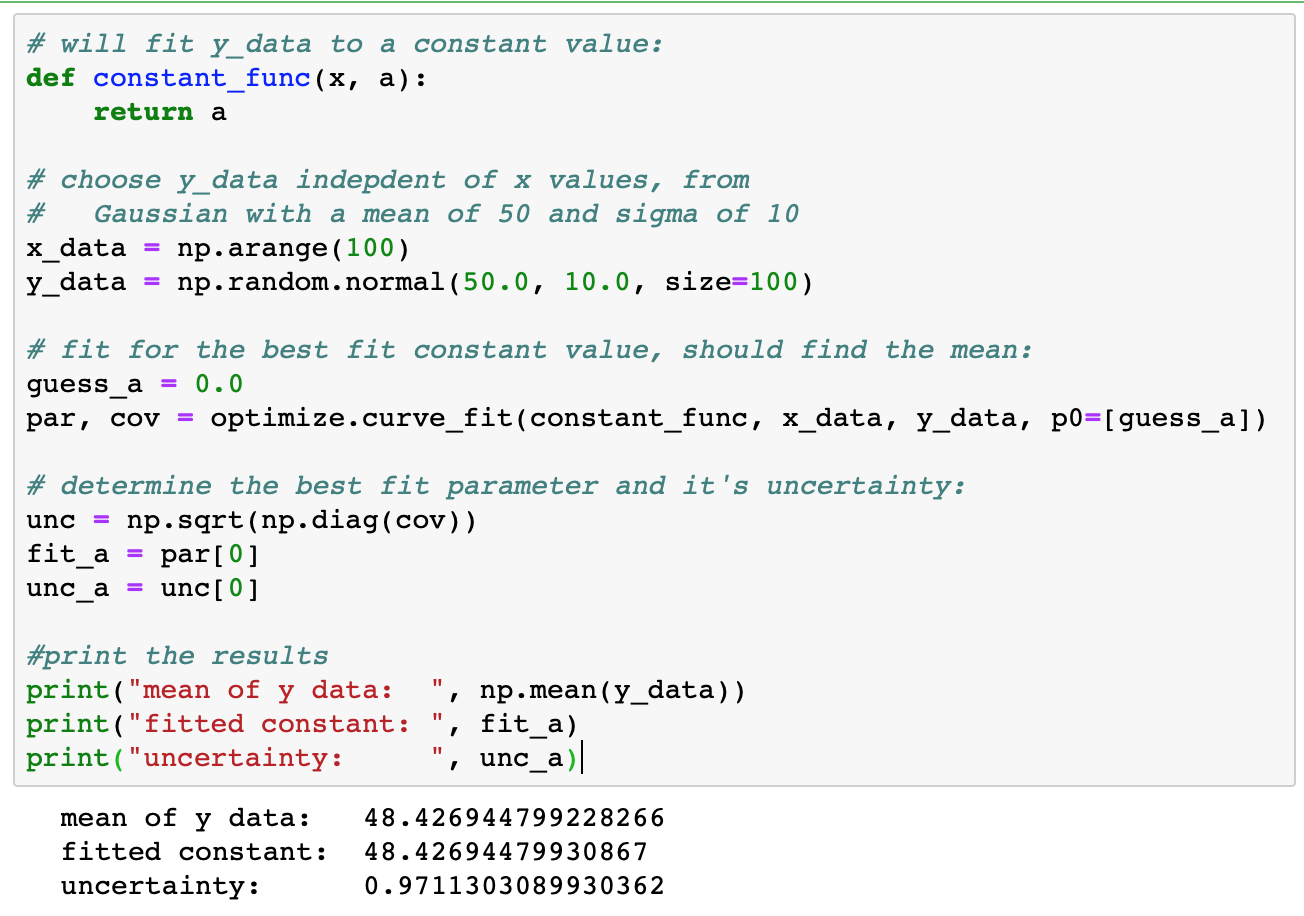
\includegraphics[width=0.65\textwidth]{figs/labs/fitting/uncertainties.png} \\
%\caption{Example obtaining parameter uncertainties.}
%\label{fig:fitunc}
%\end{center}
%\end{figure}

Lets repeat the study in~\ref{sec:sigmatrue}. Generate $x$-values as a numpy array of evenly spaced values from 0 to 99. Generate $y$-values as 100 random numbers drawn from a Gaussian distribution with mean $m = 50$ and a width $\sigma_y =10$.  Perform a fit using {\tt curve{\_}fit} function.  Leave the uncertainties on the $y$ values
unspecified and also leave parameter {\tt absolute{\_}sigma} unspecified. 

\begin{print} Print the fitted best fit value and its uncertainty. \end{print}

It's surprising actually, that the fit returns the correct
uncertainty.  Your code does not provide  the uncertainty on the $y$ parameters $\sigma_y$ to
the fit.  So how can it possible deduce the correct uncertainty
$\sigma_m = \sigma_y / \sqrt{N}$?

The answer is that behind the scenes, the {\tt curve{\_}fit} function
is being really quite clever (too clever, in my opinion, for a default
behavior!)  By default, the covariance matrix returned by the 
{\tt curve{\_}fit} function is scaled by the factor:
\begin{displaymath}
\alpha = \frac{\chi^2_{\rm min}}{\rm NDF}
\end{displaymath}
the minimum value of the $\chi^2$ divided by the number of degrees of
freedom (number of data points minus number of parameters).  As discussed in lecture that $\alpha$ is around 1 for a least-squares fit with
an appropriate model and correct uncertainties.  So nominally this
factor is one, and has no effect.  But consider what happens if the
actual uncertainties are $\sigma$ while the $\chi^2$ used in the fit assumes they
are, for example, ``1''.  In this case, the calculated $\chi^2$ is:
\begin{displaymath}
\chi^2 = \sum_i \frac{(f(x_i;p) - y_i) ^2}{1}
\end{displaymath}
which differs from the correct $\chi^2$:
\begin{displaymath}
\chi^2 = \sum_i \frac{(f(x_i;p) - y_i) ^2}{\sigma^2}
\end{displaymath}
by a factor of $\sigma^2$.  This means that while the correct value
for $\alpha$ is nearly one, the calculated value of alpha will be
$\sigma^2$.  This is precisely the factor needed to scale the squared
parameter uncertainties to account for the fact that the initial
uncertainty was $\sigma$ but we assumed $1$.

This behavior is controlled by the parameter {\tt absolute{\_}sigma}.
By default, the function sets {\tt absolute{\_}sigma = False} and
scales the covariance matrix as just described.  On the other hand, if
you want to simply use the provided uncertainties without re-scaling
the covariance matrix, you must remember to set {\tt
  absolute{\_}sigma = True}.  I think this is a really poor choice of
default behavior...  it's really quite a fancy thing to do implicitly.
In cases when you know the uncertainty on your data points, this
re-scaling actually results in less correct estimate for the
uncertainties.  This is because for a good model with proper
uncertainties, the factor $\alpha$ is near one, but not exactly one.

\begin{print} Repeat the study but leave the uncertainties on the $y$ values
unspecified and set {\tt absolute{\_}sigma = True} in the fit.  You
should obtain an uncertainty of $0.1$.  Print your value and print your explanation of
why you obtained this value. \end{print}

As a rule of thumb, when using {\tt curve{\_}fit}, if you provide
explicit uncertainties, you should remember to set {\tt
  absolute{\_}sigma = True}.  And really, for precision work, you should
almost always be providing explicit uncertainties.



















% fourier
%\chapter{The Central Limit Theorem and Experimental Uncertainties}

%
% TODO:  Students were confused about how to handle bin position
% for plotting discrete data...  some clarification (text, figures) is needed.
%

\section{Introduction}

In this lab, you will produce a numerical demonstration of the central
limit theorem.  You will also model the propagation of uncertainties
and compare with the calculated uncertainties. For this lab there are only jupyter notebook entries. 


\section{Sampling Distributions}

\begin{figure}[htbp]
\begin{center}
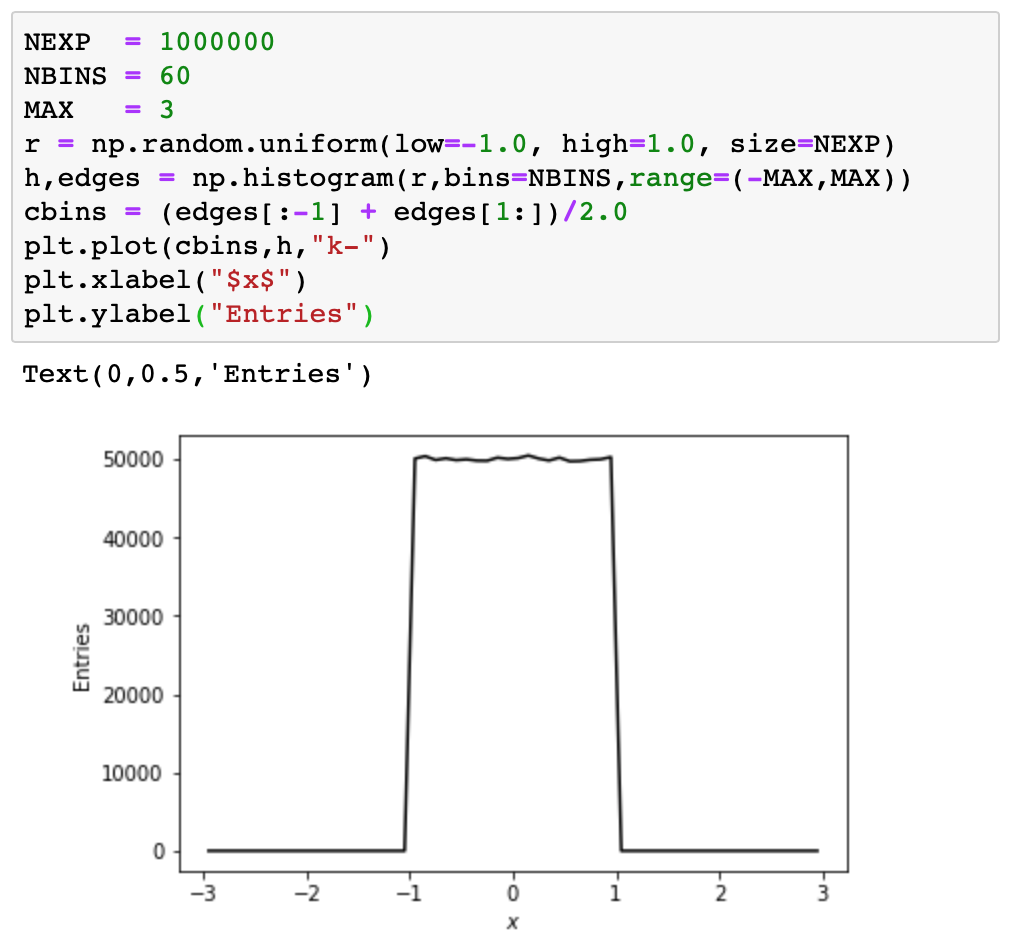
\includegraphics[width=0.75\textwidth]{figs/labs/uncertainties/step.png}\\
\end{center}
\caption{\label{fig:samplingstep} Sampling from the uniform distribution. }
\end{figure}

\begin{figure}[htbp]
\begin{center}
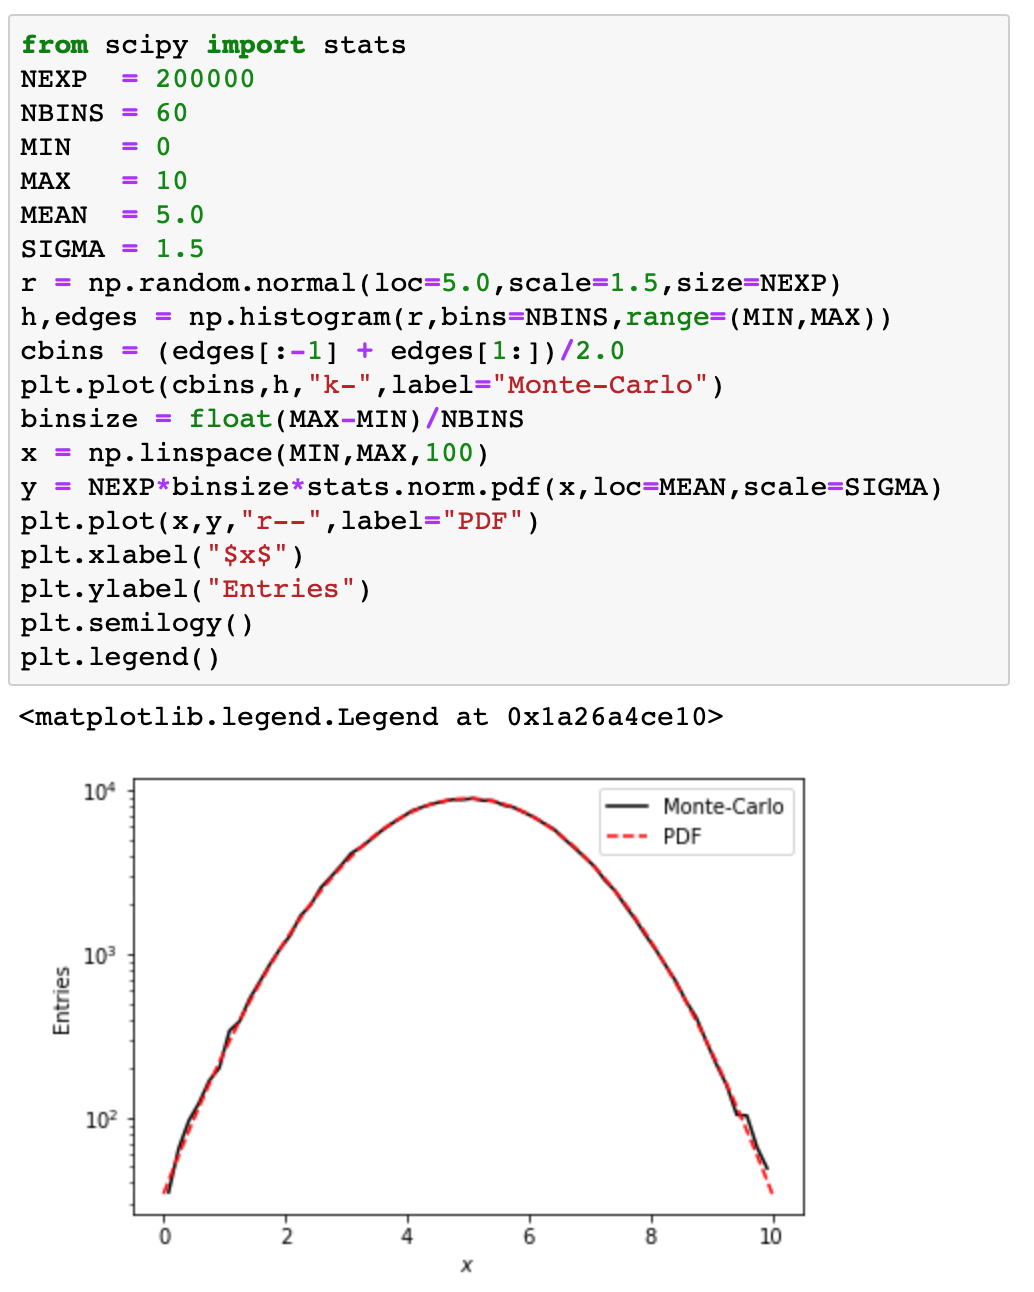
\includegraphics[width=0.75\textwidth]{figs/labs/uncertainties/gaussian.png}\\ 
\end{center}
\caption{\label{fig:samplinggauss} Sampling from the Gaussian distribution and comparison with the Gaussian PDF.}
\end{figure}

Scientific python provides functions to draw random samples according
to various distributions.  In today's lab, we will draw samples
uniformly in the interval $[-1,1]$, as demonstrated in Fig.~\ref{fig:samplingstep}.   The line
\begin{verbatim}
r = np.random.uniform(low=-1.0, high=1.0, size=NEXP)
\end{verbatim}
creates a NumPy array {\tt r} which contains {\tt NEXP} entries, with
each entry chosen uniformly and randomly in the range from -1 to 1.
In the example, these events are displayed in a histogram.  When
plotting histograms with plenty of statistics (one million entries
here) and fine binning (60 bins here) it is usually preferable to use
lines instead of points with error bars for plotting the histograms,
as is done in this example.  Notice, however, that even with one
million events, there are still statistical fluctuations which prevent
the curve from being perfectly smooth.

In Fig.~\ref{fig:samplinggauss}, entries are instead drawn from the Gaussian distribution with the line:
\begin{verbatim}
r = np.random.normal(loc=5.0,scale=1.5,size=NEXP).
\end{verbatim}
The histogram is plotted with a logarithmic $y$ scale:
\begin{verbatim}
plt.semilogy()
\end{verbatim}
which results in the Gaussian distribution appearing as a parabola.  The histogram is compared to the Gaussian PDF appropriately normalized:
\begin{verbatim}
x = np.linspace(MIN,MAX,100)
y = NEXP*binsize*stats.norm.pdf(x,loc=MEAN,scale=SIGMA)
\end{verbatim}


\section{Demonstration of the Central Limit Theorem}

In this section, you'll show that average value of random variables
chosen uniformly from -1 to 1 approaches a Gaussian distribution,
consistent with the central limit theorem.  First create a 2-D array
of size {\tt NEXP} by {\tt NAVG} filled with uniform random values in
the interval from -1 to 1, as follows:
\begin{verbatim}
r = np.random.uniform(low=-1.0, high=1.0, size=(NEXP,NAVG))
\end{verbatim}
Then calculate averages values from {\tt NAVG} entries:
\begin{verbatim}
x = np.sum(r, axis=1)/float(NAVG)  
\end{verbatim}
From the Central Limit Theorem, we expect the entries in x to approach a Gaussian distribution.

\begin{plot}  Set {\tt NEXP} to 1000000 for plenty of statistics.
Produce three different histograms with 40 bins covering the range
from -1.2 to 1.2 for three values {\tt NAVG}: 1,2, and 3.  Plot all
three histogram in the same graph with appropriate legend. \end{plot}

Your plot will show that already for three contributions to the average, the result looks quite Gaussian on a linear scale.  For more precise comparison, will use a log scale and compare to the PDF.

\begin{plot} Calculate {\tt NEXP}$=1000000$ average values {\tt x} for {\tt NAVG}$=10$.  Calculate the mean value of the entries in {\tt x} using the {\tt np.mean} function.  Calculate $\sigma$ for the entries in $x$ by taking the square root of the output from the {\tt np.var} (variance) function.  Produce a histograms with 20 bins covering the range
from -0.5 to 0.5 for the average values.  Compare with a Gaussian distribution, appropriately normalized, using your calculated values from the  mean and sigma.  Plot both the histogram and PDF on the same graph, including an appropriate legend.  Use a logarithmic $y$ axis. \end{plot}


\section{Propagation of Uncertainties}

\begin{figure}[htbp]
\begin{center}
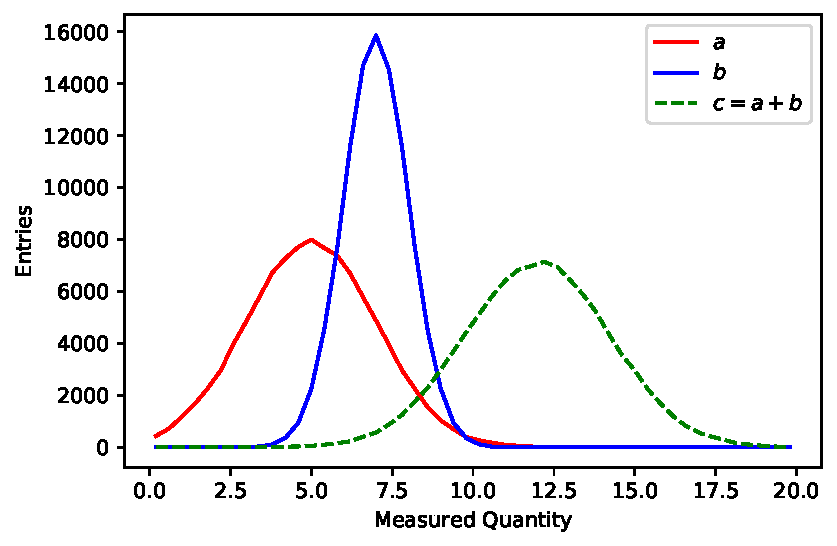
\includegraphics[width=0.75\textwidth]{figs/labs/uncertainties/addunc.pdf}\\
\end{center}
\caption{\label{fig:addunc} Simulation of many measurements of the quantity $c = a + b$. }
\end{figure}

Consider two measured values $a \pm \sigma_a$ and $b \pm \sigma_b$.  If we calculate the quantity $c = a + b$ or $c = a - b$, the uncertainty on the calculated value $c$ is given by:
\begin{displaymath}
\sigma_c = \sqrt{\sigma_a^2 + \sigma_b^2}.
\end{displaymath}
If instead, we calculate $c = a * b$ or $c = a/b$ the fractional uncertainty on $c$ is given by:
\begin{displaymath}
\frac{\sigma_c}{c} = \sqrt{\left(\frac{\sigma_a}{a}\right)^2 + \left(\frac{\sigma_b}{b}\right)^2}.
\end{displaymath}
In this section, you'll develop a numerical simulation for the
propagation of uncertainties under addition, subtraction,
multiplication, and division.  An example, for $c = a + b$ is shown in Fig.~\ref{fig:addunc}.

\begin{print} Pick values for $a$, $b$, $ \sigma_a$ and $ \sigma_b$ for simulating subtraction: $c=a-b$. Print them out in your notebook. Choose the values that are different from what is plotted in Fig.~\ref{fig:addunc}.  \end{print}

\begin{plot} 
Simulate the measurement $a$ by drawing 100,000 random variables
sampled from the Gaussian distribution with mean $a$ and sigma
$\sigma_a$, and likewise for $b$.  Calculate the values of $c = a -b $ from
the $a$ and $b$ values.  Plot the result in histogram with 50 bins and an appropriate range. \end{plot} 

\begin{print} 
Calculate the mean and variance of the mean and variance of the simulated $c$ values and compare to your expectations for the mean, variance of the distribution and variance of the mean. Apply the standard propagation of uncertainties for calculating expectation value for the variances. 
 \end{print}


This is a \textbf{sign-off point} for this lab. 

\begin{print} Pick values for $a$, $b$, $ \sigma_a$ and $ \sigma_b$ for simulating division: $c=a/b$. Print them out in your notebook.  Choose the values that are different from what is plotted in Fig.~\ref{fig:addunc}.  \end{print}

\begin{plot} 
Simulate the measurement $a$ by drawing 100,000 random variables
sampled from the Gaussian distribution with mean $a$ and sigma
$\sigma_a$, and likewise for $b$.  Calculate the values of $c = a/b $ from
the $a$ and $b$ values.  Plot the result in histogram with 50 bins and an appropriate range. \end{plot} 

\begin{print} 
Calculate the mean and variance of the mean and variance of the simulated $c$ values and compare to your expectations for the mean, variance of the distribution and variance of the mean. Apply the standard propagation of uncertainties for calculating expectation value for the variances. 
 \end{print}

 
%{\bf Plot 3-6:}  Produce four plots simulating addition, subtraction, multiplication, and division, as in Fig.~\ref{fig:addunc}.  In each case, compare the measured variance of the $c$ values with your expectation.































\end{document}

% OTHER IDEAS:
% Fourier Transforms
% Monte Carlo techniques
% Speed of Light in Cable
% Measure e from shot noise
